\documentclass[10pt,letterpaper]{article}
\usepackage{style/tmlr}
\usepackage{amsmath,amssymb,booktabs,graphicx,microtype,float}
\usepackage{hyperref}
\hypersetup{hidelinks,pdftitle={Evaluating the Deployment Utility of a Frozen Policy-Update Procedure: Scale, Completion Preference, and Joint Evidence},pdfauthor={},pdfkeywords={Deployment Utility, Policy-Update Evaluation, Proxy-Based Selection, Completion Preference, Joint Statistical Inference, Execution Simulation}}
\newcommand{\E}{\mathbb{E}}
\newcommand{\Prob}{\mathbb{P}}
\graphicspath{{figures/}}
\title{Evaluating the Deployment Utility of a Frozen Policy-Update Procedure: Scale, Completion Preference, and Joint Evidence}
\author{Anonymous authors\thanks{Code and saved-outcome data are available at \url{https://github.com/computational-decision-lab/deployment-utility-evaluation}; release \texttt{202611050855}.}}
\date{}
\begin{document}
\maketitle
\footnotetext{\textbf{Reproducibility.} Code and saved-outcome data are available at \url{https://github.com/computational-decision-lab/deployment-utility-evaluation}; dated release \texttt{202611050855}.}
\begin{abstract}
Policy updates selected by proxy scores need not yield positive operational utility when the complete selection and adoption procedure is deployed. We define procedure-level deployment utility as expected incumbent-relative utility under stated operating conditions, including incumbent-retaining decisions. We characterize three elementary properties: reversal frequency alone does not determine mean procedure utility; fixed-selection revaluation under affine completion utility yields a linear preference frontier; and repeated deployments reduce within-root noise without increasing the number of independent roots. These characterizations introduce no new fidelity metric or inference algorithm. We instantiate the assessment for a frozen execution-policy procedure in a synthetic continuous double auction. Fifty independent roots each generate a shared pool of 16 candidates, followed by one proxy-based selection per root--regime pair (100 selection decisions) and paired evaluations on separate interactive books across two liquidity regimes, three order sizes, and two inventory-response settings. Under the prespecified 100-basis-point completion preference and approximate simultaneous bands for the original 24-estimate family, all four largest-scale means are negative, while lower-scale means and response and interaction contrasts remain unresolved. Fixed-selection revaluation over four preferences shows that the deployment conclusion depends on utility and inferential-family choice; at 100 basis points, the same liquid-regime estimates include zero in the wider 64-estimate diagnostic family. A separate outcome-aware diagnostic at the selection scale estimates positive proxy-minus-deployment gaps of 0.95--1.31 bps across four regime--response cells, with a separate simultaneous band; because it combines winner selection, finite proxy-sample noise, and replay versus interactive worlds, it is not a causal estimate of proxy bias. An exploratory post-outcome fixed-selection diagnostic estimates break-even preferences with uncertainty reported separately. The study provides bounded empirical evidence and an auditable reporting specification. It establishes neither general agent reliability, a universal scaling law, nor real-market execution validity.
\end{abstract}

\section{Introduction}
Machine-learning systems increasingly generate candidate policies, models, or programs and use proxy evaluations to choose updates before deployment. The selected candidate's proxy score is not the operational utility of the complete procedure that generated and selected it. Procedure-level utility also depends on whether an update is adopted, the conditions under which the deployed system operates, how outcomes are valued, and the population of independent update decisions to which the estimate is meant to generalize. Retaining the incumbent is one possible output of the procedure, not a missing observation.

Several established directions address parts of this problem. Off-policy evaluation estimates a target policy's value from data generated by another policy \citep{jiang2016,thomas2015}; safe policy improvement studies how to construct updates with guarantees relative to a baseline \citep{laroche2019}; and the closest TMLR precedent, \citet{abdelwahed2024conservative}, uses conservative off-policy value estimates to inform deployment of offline-learned policies. Active offline policy selection allocates limited online interaction adaptively across candidate policies \citep{konyushkova2021active}. Agent-evaluation work studies benchmark coverage and the reliability of model, scaffold, and task comparisons \citep{kapoor2026,hardy2026,kehkashan2026}. These works motivate careful deployment assessment, but their principal targets differ from ours: we estimate incumbent-relative utility of a complete frozen update-selection procedure, including adoption and no-update decisions, on fresh interactive deployments.

We use \emph{procedure-level deployment utility} for the expected incumbent-relative utility of a frozen update-selection procedure under declared operating conditions and an explicit utility. Its assessment specifies the procedure, adoption rule, independent-root population, deployment conditions, utility, and inferential family. It separates three questions: whether a selected candidate improves on a proxy, whether the complete procedure has positive expected utility, and whether the independent evidence supports a deployment claim. The resulting assessment specification organizes existing design and statistical choices; it is not a new universal metric, selection algorithm, or general theory.

We instantiate this assessment in a synthetic continuous double auction. A frozen replay-proxy procedure selects among a fixed pool of 16 candidates per root, after which selected policies and incumbents are compared on separate interactive books. The principal design varies order scale, liquidity regime, and inventory-response condition over a shared population of 50 independent generation roots. It is a controlled evaluation substrate, not a calibrated professional market. The candidate-pool size is fixed, so this paper does not estimate how search pressure changes with the number of candidates.

Two research questions organize the evidence. \textbf{RQ1:} How does operating scale affect the expected utility of the frozen update-selection procedure under a prespecified utility? \textbf{RQ2:} How does fixed-selection revaluation across completion preferences change estimated utility, and how does inferential-family choice change the evidence supporting a deployment claim? The original market analysis addresses RQ1. Utility revaluation and the break-even analysis address RQ2 as post-outcome diagnostics. Root deletion and alternative bands are sensitivity audits of the same cohort, not independent confirmation.

The paper makes three bounded contributions. First, it states the procedure-level estimand and gives three elementary decision-theoretic and sampling properties that clarify magnitude dependence, utility frontiers, and the role of independent roots; these are formal characterizations, not a new estimator or nontrivial general theorem. Second, it reports a separately frozen interactive-market cohort with 50 shared independent roots, 100 selection decisions, 2,400 paired deployment records, and a prespecified 24-estimate inferential family. Third, it provides an auditable reporting specification that binds the procedure, adoption rule, population, operating conditions, utility, and evidence family, alongside reproducible saved-outcome reanalysis.

Under the original 100 bps completion preference and approximate simultaneous bands for the 24-estimate family, the four largest-scale procedure means are negative. Lower-scale cell means and response and interaction contrasts remain unresolved. At 100 bps, the liquid-regime point estimates are unchanged but their intervals include zero in the wider 64-estimate diagnostic family. A separate post-outcome comparison at the $s=0.05$ selection scale estimates positive proxy-minus-deployment gaps of 0.95--1.31 bps across four regime--response cells; this auxiliary family does not identify causal proxy bias. This evidence is conditional on one frozen procedure and synthetic market. A restricted planner-code case with only three generation roots is retained as an auxiliary result in the Supplementary Material and does not support broad agent generalization.

\section{Related work and contribution boundary}
\subsection{Policy evaluation and safe improvement}
Off-policy evaluation estimates the value of a target policy from logged trajectories generated by another policy. Doubly robust evaluation combines importance weighting and value modeling for this setting \citep{jiang2016}; high-confidence off-policy evaluation constructs a lower confidence bound for a policy's expected return from logged trajectories \citep{thomas2015}. Safe Policy Improvement with Baseline Bootstrapping (SPIBB) addresses a constructive problem: it uses a baseline policy where evidence is insufficient to seek policy improvement with safety guarantees \citep{laroche2019}. The closest TMLR precedent is \citet{abdelwahed2024conservative}, which uses conservative off-policy policy-value evaluation and confidence bounds to support a deployment decision for offline-learned policies. Our target is different: rather than evaluating only a fixed learned policy or proposing a safe-improvement algorithm, we estimate the expected incumbent-relative utility of the complete frozen generation, proxy-selection, adoption, and incumbent-retention procedure. The present study uses separate interactive deployment evaluations; it does not propose an off-policy estimator or a safe-improvement guarantee.

\subsection{Policy selection under limited online evaluation}
\citet{konyushkova2021active} combine logged-data off-policy estimates with a limited online-interaction budget, then use Bayesian optimization to choose which candidate policy to evaluate next. This is an adaptive allocation problem: the evaluation sequence changes in response to earlier observations. We instead freeze the 16-candidate proxy-selection and adoption procedure, evaluate its resulting choices on fresh paired deployments, and estimate procedure-level utility across operating scales and completion preferences. We do not optimize the interaction budget or compare adaptive evaluation strategies.

\subsection{Stable policy learning and sampling risk}
\citet{stable2026} study how algorithmic stability shapes the tradeoff between expected welfare and sampling risk when a policy is learned from an experimental sample and then implemented at scale. They propose policy-vote bagging and derive bounds linking estimation accuracy, subsample size, and welfare variation, including an exact guarantee under CARA utility. Their target is the stability and welfare risk of the learning algorithm under sample perturbations. Our target is different: we freeze candidate generation, proxy selection, adoption, and incumbent retention, then evaluate incumbent-relative utility on fresh interactive deployments across declared conditions. We do not measure sampling risk in the Stable Policy Learning sense, and we keep this confirmatory assessment distinct from post-outcome diagnostics.

\subsection{Agent evaluation and measurement reliability}
The Holistic Agent Leaderboard (HAL) develops evaluation infrastructure and compares models, scaffolds, and benchmarks across 21,730 rollouts \citep{kapoor2026}. \citet{hardy2026} decompose variation in agent rankings across models, scaffolds, and tasks and show that evaluation reliability depends on the intended ranking claim. A broader review reports gaps between task-success metrics and deployment-relevant dimensions in the benchmarks it surveys \citep{kehkashan2026}. This work primarily assesses agent capabilities, benchmark infrastructure, or ranking reliability. We instead target the expected incumbent-relative utility of a procedure that generates and selects updates; the independent population is update-generation roots under a specified frozen design, not a population of models or tasks. The completion preference in our market utility is not a measure of API cost, compute efficiency, or safety.

\subsection{Proxy optimization and selection bias}
Optimizing an imperfect reward proxy can increase its discrepancy from a reference reward, while reward-model ensembles address this effect in the studied reinforcement-learning settings \citep{gao2022,coste2024}. Model-selection bias and adaptive leaderboard submissions provide related accounts of evaluation reuse and selection effects \citep{cawley2010,blum2015}. These works motivate separating proxy selection from subsequent deployment evaluation. Our main cohort fixes the candidate pool at 16 and does not compare pool sizes, so it estimates no search-pressure effect or search-scaling law. Utility sensitivity also holds the selected policies fixed; it does not assess re-selection under alternative completion preferences.

\subsection{Policy-dependent worlds and market simulation}
Performative prediction studies settings in which model deployment changes the distribution used to measure performance \citep{perdomo2020}; WILDS organizes evaluation under specified distribution shifts \citep{koh2021}. In financial simulation, recent work studies calibration, endogenous order flow, and the response of generated limit order books to injected orders \citep{noble2026,nigmatulin2026}. These works examine related but distinct objects: distributional response, robustness, or simulator realism. Our estimate is conditional on one controlled synthetic world and does not identify real-market execution impact or certify simulator fidelity.

\subsection{Relationship to prior Improvement Fidelity work}
\citet{pivot} define Improvement Fidelity and transition-level summaries, study operator and world-response effects, and propose PIVOT-KG to allocate high-fidelity queries according to decision relevance. Their supplementary code also contains virtual execution/participation examples. In the PIVOT E6 financial fixtures, a specified position-size change is assessed on supplied historical price paths using replay and formula-based virtual fills with participation/impact parameters. Here, one frozen replay-selection procedure chooses among 16 candidates per root and is evaluated on event-driven continuous-double-auction books. The cohorts, outcome files, execution mechanisms, and inferential targets differ; the earlier financial results are not reused as current evidence. We inherit and attribute relevant evaluation concepts and standard paired/bootstrap operations, but add no new fidelity metric, validation allocator, or transition-level theorem. The present contribution is procedure-level deployment utility under operating conditions and completion preferences. Table~\ref{tab:boundary} states the substantive boundary. An anonymous copy of the actual related conference manuscript is supplied for comparison.

\begin{table}[t]\centering\small
\begin{tabular}{@{}p{.19\linewidth}p{.35\linewidth}p{.39\linewidth}@{}}\toprule
Aspect & Related PIVOT work & This study\\\midrule
Research target & Fidelity of proposed transitions and allocation of validation evidence & Deployment utility of a fixed selection procedure under scale and completion preferences\\
Method role & Fidelity quantities and PIVOT-KG & Inherited quantities and standard resampling; no new allocator\\
Market material & Fixed updates on historical price paths with formula-based virtual fills and impact & Replay-selected candidates on event-driven matching-engine books; 50 shared roots\\
Empirical claims & Game/response and validation-allocation results, including driving stress tests & Original 24-estimate deployment family; separate utility and root diagnostics\\
Auxiliary evidence & Prior manuscript's own experiments & Distinct three-root planner-code study, reported only in the supplement\\\bottomrule
\end{tabular}
\caption{Scope distinction based on the related manuscript and its submitted supplementary archive. Shared motivation and inherited methods are acknowledged; the current experiments are not offered as evidence for a new PIVOT algorithm.}\label{tab:boundary}
\end{table}

The exchange uses a pinned, unmodified PythonMatchingEngine implementation \citep{pythonmatchingengine}. Its engine lineage differs from ABIDES \citep{byrd2019,amrouni2021}. The surrounding policies, generator, and completion utility intentionally retain compatibility with our earlier development implementation. Thus, engine independence does not mean that every modeling choice was developed independently. Those development results are not part of this paper's empirical evidence.

Market-simulation research addresses a complementary validation problem. \citet{noble2026} calibrate queue-reactive state and event-time distributions from market data and introduce trade-flow feedback for impact and reversion. The LOB-Impact Benchmark injects metaorders into five autoregressive generators across five NASDAQ stocks to assess own-order response and subsequent relaxation \citep{nigmatulin2026}. These studies examine whether simulated execution dynamics are credible. We instead estimate the utility of the procedure producing a deployed policy, conditional on a specified synthetic world. The market is an evaluation environment, not a claimed new or calibrated market-impact model.

\section{Formal target and characterizations}
\subsection{Frozen procedures, adoption, and utility}
Let $R$ index an independent generation and evaluation root. A fixed procedure $\mathcal P$ generates candidates, evaluates them using pre-deployment information $H_R$, selects a provisional candidate $\widetilde\pi_R$, and decides whether to replace an incumbent $\pi_{0,R}$. Write the actual adoption event as $A_R=a(H_R)$ and the deployed policy as $\widehat\pi_R=\widetilde\pi_R$ on $A_R$, otherwise $\widehat\pi_R=\pi_{0,R}$. The adoption gate is frozen using pre-deployment information and is not conditioned on the deployment outcomes used to estimate reversal risk.

For deployment condition $z$ and utility $U_p$, define a root's conditional mean gain
\begin{equation}
g_R(z;p)=\E_\omega\left[U_p\{\widehat\pi_R,W_z(\widehat\pi_R,\omega)\}
-U_p\{\pi_{0,R},W_z(\pi_{0,R},\omega)\}\mid H_R\right],
\label{eq:root-gain}
\end{equation}
where $W_z$ denotes the policy-dependent deployment world and $\omega$ its fresh exogenous randomness. A common exogenous stream couples the two branches; each branch has its own evolving book. Matching streams does not force endogenous paths or fills to agree. If the incumbent is retained, the gain is exactly zero.

Our primary estimand is the procedure mean utility
\begin{equation}
\mu_{\mathcal P}(z;p)=\E_R[g_R(z;p)].\label{eq:procedure}
\end{equation}
The expectation includes the randomness of candidate generation and selection under the declared procedure. It excludes changes to that procedure, simulator misspecification, and research costs unless those costs are part of $U_p$. The market utility here does not charge for generating or validating candidates. The experiment therefore evaluates deployment value, not the net profitability of conducting the research programme.

An adoption-conditioned reversal probability, $\Prob\{g_R(z;p)<0\mid A_R\}$, is a complementary inherited risk description \citep{pivot}. It is undefined when adoption probability is zero. No-update outcomes remain in $\mu$, and
\begin{equation}
\mu_{\mathcal P}(z;p)=\Prob(A_R)\E_R[g_R(z;p)\mid A_R]
\label{eq:adoption-identity}
\end{equation}
when $\Prob(A_R)>0$.

\paragraph{Formal characterization 1 (Magnitude dependence).}
Let $q=\Prob(A_R)>0$, let $G_R=g_R(z;p)$ on $A_R$, and define $G_+=\max(G_R,0)$ and $G_-=\max(-G_R,0)$. Then
\begin{equation}
\mu_{\mathcal P}(z;p)=q\left\{\E[G_+\mid A_R]-\E[G_-\mid A_R]\right\}.
\label{eq:magnitude-decomposition}
\end{equation}
Consequently, adoption and reversal frequencies alone do not determine procedure utility; the magnitudes of adopted gains and losses are also required. \emph{Proof.} Condition on $A_R$ in Equation~\ref{eq:adoption-identity} and write $G_R=G_+-G_-$. For example, with $q=1/2$, adopted gains $+2$ and $-1$ give mean $0.25$, whereas replacing the loss with $-10$ gives mean $-2$; both have conditional reversal frequency $1/2$. \hfill$\square$

In the market data, each root gain is estimated using four deployment repetitions. Reported reversal counts use the sign of that estimated root mean, with the recorded $10^{-9}$ bps numerical tolerance. They are descriptive observed-root sign counts, not noise-corrected estimates of the latent conditional probability above, and have no simultaneous risk guarantee.

\subsection{Deployment-utility assessment specification}
The report can be indexed by $\mathcal D=(\mathcal P,A,\mathcal R,z,U_p,F)$, where $R\sim\mathcal R$ identifies the independent root population and $F$ the family of claims assessed jointly. This notation collects the design choices underlying Equation~\ref{eq:procedure}; it introduces no new estimand. Table~\ref{tab:specification} maps the specification to the principal experiment. In particular, 50 is the number of sampled roots, not the definition of the target population.

\begin{table}[t]\centering\small
\begin{tabular}{@{}p{.18\linewidth}p{.32\linewidth}p{.43\linewidth}@{}}\toprule
Element & Question to specify & Principal experiment\\\midrule
Procedure $\mathcal P$ & How are updates produced and chosen? & Frozen generator, 16 candidates, replay-proxy selection\\
Adoption $A$ & When is the incumbent replaced? & Proxy gain exceeds $10^{-9}$ bps; otherwise retain it\\
Population $\mathcal R$ & Which independent decisions are represented? & Roots from the frozen generator/world design; 50 sampled roots shared across regimes\\
World $W_z$ & Where will the decisions operate? & Two liquidity regimes, three order sizes, two response settings\\
Utility $U_p$ & How are operational outcomes valued? & Shortfall and unfinished fraction; primary $p=100$ bps\\
Estimand $\mu_{\mathcal P}$ & What average utility is sought? & Incumbent-relative gain of the whole procedure, including no-update zeros\\
Evidence $F$ & Which claims share uncertainty control? & Original 24 estimates; 20,000 whole-root bootstrap draws\\\bottomrule
\end{tabular}
\caption{Deployment-utility assessment specification. The general questions can be reused with other procedures and utilities; their empirical validation here is confined to the stated studies.}\label{tab:specification}
\end{table}

A prospective application freezes candidate generation, selection, and adoption; declares deployment conditions, utility, and the root population; and fixes the inferential family before examining outcomes. It then estimates paired gains, retains incumbent decisions, and reports joint evidence with completeness and sensitivity audits. Any outcome-aware revision receives a separate diagnostic identity. This workflow organizes standard evaluation operations, rather than establishing their validity in an untested domain.

\begin{table}[t]\centering\small
\begin{tabular}{@{}p{.12\linewidth}p{.78\linewidth}@{}}\toprule
Stage & Frozen assessment procedure\\\midrule
Input & Freeze candidate generation, proxy selection, adoption rule, incumbent, target root population, deployment conditions, utility, and inferential family.\\
1 & For each independent root, generate candidates and select a provisional update using only pre-deployment proxy information.\\
2 & Apply the frozen adoption rule; record an incumbent-retaining decision as a zero procedure gain.\\
3 & For each declared deployment condition, evaluate selected and incumbent policies on fresh paired deployments, keeping the complete root vector.\\
4 & Average deployment repetitions within root; estimate the procedure mean and construct joint evidence by resampling whole roots across the declared family.\\
Output & Report estimates, uncertainty, completeness, sensitivity analyses, and the scope of any deployment interpretation.\\\bottomrule
\end{tabular}
\caption{Operational steps for a procedure-level deployment assessment. The statistical operations are standard; the contribution is an explicit reporting target and its bounded empirical application.}\label{tab:assessment-procedure}
\end{table}

\subsection{Decision-theoretic and sampling properties}
For the affine completion utility used in the market, define
\begin{equation}
U_p=-S-pf, \qquad
a_z=\E_R[S_{\rm incumbent}-S_{\rm selected}], \qquad
b_z=\E_R[f_{\rm incumbent}-f_{\rm selected}],
\label{eq:utility-components}
\end{equation}
where expectations include fresh deployment randomness and no-update roots. Fixed selections therefore satisfy
\begin{equation}
\mu_{\mathcal P}(z;p)=a_z+p b_z.
\label{eq:utility-frontier}
\end{equation}

\paragraph{Formal characterization 2 (Fixed-selection utility frontier).}
Under Equation~\ref{eq:utility-components}, the procedure mean is affine in $p$. If $b_z\ne0$, its mathematical zero is $p_z^*=-a_z/b_z$. Thus changing $p$ can change the assessed utility without changing any selected policy or deployment outcome; it does not evaluate re-selection under the new preference. \emph{Proof.} Subtract the incumbent and selected utilities and take expectations: $\E[-S_{\rm selected}-pf_{\rm selected}+S_{\rm incumbent}+pf_{\rm incumbent}]=a_z+p b_z$. Solving $a_z+p b_z=0$ gives the stated zero.\hfill$\square$

For inference, let $C_z\subseteq\mathbb R^2$ be a joint confidence set for $(a_z,b_z)$. The corresponding projected zero set is
\begin{equation}
\mathcal P_z^*(C_z)=\left\{p\geq0:\exists(a,b)\in C_z,\ a+pb=0\right\}.
\label{eq:zero-set}
\end{equation}
A conservative sign classification at preference $p$ can use
\begin{equation}
\underline\mu_z(p)=\inf_{(a,b)\in C_z}(a+pb), \qquad
\overline\mu_z(p)=\sup_{(a,b)\in C_z}(a+pb).
\label{eq:utility-support}
\end{equation}
The set in Equation~\ref{eq:zero-set} is reported only for the separate outcome-aware break-even diagnostic in Section~\ref{app:break-even}; it is not part of the original 24-estimate family. If $\underline\mu_z(p)>0$, the confidence set supports a positive mean; if $\overline\mu_z(p)<0$, it supports a negative mean; otherwise the sign remains unresolved, conditional on the stated coverage event.

\subsection{Joint evidence across deployment conditions}
For regime $g$, response $\rho$, and scale $s$, average the four paired repetitions within root $r$:
\begin{equation}
D_{r,g,\rho,s}=\frac14\sum_{k=1}^4
\left(U_{r,g,\rho,s,k}^{\rm selected}-U_{r,g,\rho,s,k}^{\rm incumbent}\right).
\end{equation}
Each root contributes its complete vector of cell gains and contrasts. Both regimes use the same 50 roots, so the independent sample size is 50, not the 100 root--regime decisions or the 2,400 paired repetitions. The population interpretation assumes independently generated roots from the frozen design. Shared regimes and repeated deployments improve within-root comparisons without adding independent roots.

The original inferential family contains 12 cell means, four largest-minus-smallest scale contrasts, six response contrasts, and two scale-by-response interactions. For root vector $X_r\in\mathbb R^{24}$, let $\overline X$ be its sample mean. Each of 20,000 bootstrap draws resamples 50 whole root vectors with replacement and computes
\begin{equation}
T_b=\max_{1\leq j\leq24}|\overline X^{(b)}_j-\overline X_j|.
\end{equation}
The empirical 95th percentile $q$ gives the bands $[\overline X_j-q,\overline X_j+q]$. This is the prespecified unstandardized maximum-deviation construction, with approximate simultaneous coverage conditional on the experiment. It is not an exact small-sample guarantee. All 24 estimands are retained even when the main text highlights only a subset.

\paragraph{Formal characterization 3 (Independent-root target and variance decomposition).}
For a fixed deployment condition, suppose $D_{R,1},\ldots,D_{R,m}$ are conditionally independent paired deployment gains given the frozen pre-deployment information $H_R$, with conditional mean $g_R$ and variance $\sigma_R^2$. Define $\widehat g_R=m^{-1}\sum_kD_{R,k}$ and $\widehat\mu_{\mathcal P}=n^{-1}\sum_{r=1}^n\widehat g_r$ over independent roots. Then
\begin{equation}
\E[\widehat\mu_{\mathcal P}]=\mu_{\mathcal P}, \qquad
\operatorname{Var}(\widehat\mu_{\mathcal P})
=\frac{\operatorname{Var}_R(g_R)}{n}
 +\frac{\E_R[\sigma_R^2]}{nm}.
\label{eq:variance-decomposition}
\end{equation}
\emph{Proof.} Conditional independence gives $\E[\widehat g_R\mid H_R]=g_R$ and $\operatorname{Var}(\widehat g_R\mid H_R)=\sigma_R^2/m$. Apply iterated expectation and the law of total variance to the mean of $n$ independent root-level estimates.\hfill$\square$

This decomposition makes the inferential unit explicit: increasing $m$ reduces within-root deployment noise, whereas increasing $n$ reduces both root-population and within-root contributions. The 2,400 paired records in the market study therefore do not constitute 2,400 independent observations; the primary independent unit is the 50-root cluster.

For an ordered scale grid, a positive initial segment requires every included cell's joint lower bound to exceed the numerical tolerance. Its length is zero if the first cell is unresolved. An upper bound above zero merely fails to exclude positive value. Neither summary supplies a continuous capacity threshold, monotonicity between scales, or a guarantee about every adopted update. Constant empirical columns require special care: a degenerate bootstrap is not proof of absent population variation. The common radius in this experiment also applies to the observed constant columns.

\section{Empirical instantiation: a frozen procedure in a synthetic market}
The experiment instantiates the assessment specification in a controlled execution environment. Its target is one frozen procedure's value at the declared operating conditions. The grid and root population delimit the claim; they do not establish a general law of agent deployment or market capacity.
\subsection{World, policies, and selection}
The protocol was frozen on September 30, 2026, after background calibration and before this cohort's candidate selection and deployment outcomes. It binds the source, engine revision, random-stream scheme, candidate rule, utility, scale grid, and inferential family. This is a recorded prospective freeze for the cohort, not an external preregistration or a claim that prior development played no role.

The 50-root sample size and three workload fractions are fixed features of that protocol, not values selected after a significance check. Shared roots couple the regime comparisons and keep candidate-generation variation matched. They therefore require a shared-cluster analysis. The 24-estimate family covers every cell and the planned scale, response, and interaction contrasts, rather than only the most favorable comparisons. The recorded design supplies no power guarantee for effects or populations outside that family.

The world contains six liquidity providers and twelve background takers. Each provider maintains five bid and five ask levels. Liquid-regime quotes have 100 shares per level, a two-tick half-spread, and a five-second mean refresh time; the thin regime uses 20 shares, four ticks, and 15 seconds. Background takers submit ten-share immediate-or-cancel orders on independent clocks with a 12-second mean interval and equally likely sides. A fundamental price starts at 10,000 ticks and takes symmetric one-second innovations. These settings describe a synthetic population and were not fitted to a trading venue.

A path lasts 540 seconds. The buy execution parent arrives at second 120 and makes seven decisions, 60 seconds apart, through second 480. Eighty background-only calibration paths determine expected volume during the execution window: 6,252 shares in the liquid regime and 4,239 in the thin regime. Parent size is $Q=\operatorname{round}(sV_g)$ for $s\in\{0.002,0.05,0.30\}$. Scale therefore denotes a fraction of calibrated background volume, not the realized participation fraction of every execution path.

Inventory response $\rho\in\{0,1\}$ shifts a provider's quote center by a clipped function of the inventory change since parent arrival. When $\rho=0$, this channel is disabled; executions still change book depth and later fills. Quote quantities, widths, refresh clocks, and requested submission counts are fixed across response settings. The response intervention neither represents a fully learning opponent nor disables all endogenous market effects in its zero setting.

For each of 50 roots, the frozen generator produces 16 local policy perturbations and reuses the pool in both regimes. Eight proxy backgrounds per regime evaluate every candidate against the incumbent at scale 0.05. The replay proxy executes against displayed snapshots without allowing the focal execution to change subsequent books. The recorded proxy gain and interactive utility use the same $U_{100}$ accounting convention, although replay does not reproduce the policy-dependent book changes in deployment. The greatest average paired gain wins, with deterministic index tie breaking. A candidate is adopted only when its gain exceeds $10^{-9}$ bps; otherwise the procedure retains the incumbent. All 100 root--regime choices close before interactive deployment. The experiment provides no market search-pressure contrast.

Every child order has immediate-or-cancel semantics, including limited-price children; the policy class does not model a persistent passive order waiting in a queue. Candidate generation and policy equations are compatible with earlier development code, while the exchange and this cohort are separately bound. Appendix~\ref{app:protocol} gives further parameters and the provenance boundary.

\subsection{Utility and completion preference}
Let $S$ be execution implementation shortfall in bps and $f$ the unfinished fraction of the parent. The primary utility is
\begin{equation}
U_{100}=-S-100f.\label{eq:utility}
\end{equation}
A no-fill episode has saved null shortfall, interpreted as zero in this convention, and utility $-100$ bps. The coefficient expresses a preference for completing the order; it is not an estimated market price of noncompletion. At fixed shortfall, one additional percentage point unfinished reduces utility by one bps. The coefficient was inherited from development and frozen before the present cohort's selections. It was not selected to make this cohort's result negative.

For a diagnostic coefficient $p$, keep the selected policies and their saved execution outcomes fixed. The resulting paired difference is
\begin{equation}
\Delta_p=(S_{\rm incumbent}-S_{\rm selected})
+p(f_{\rm incumbent}-f_{\rm selected}).\label{eq:revalue}
\end{equation}
This accounting equation changes the valuation of observed execution, not the selection policy. A procedure that selected candidates using $p=25$ could choose different policies, which these saved outcomes alone do not evaluate. Throughout the revaluation, $\mathcal P$ remains the procedure originally selected using $p=100$.

\subsection{Completeness and accounting checks}
The cohort contains all 1,200 prescribed background checks, 100 completed choices, and 2,400 paired deployment repetitions. No failed root was replaced to reach the planned count. In 98 choices an update was adopted; the other two retain zero gain at every cell. Those two choices allow identical incumbent/selected branches to share verified episode artifacts, yielding 4,752 live episodes rather than the nominal 4,800.

Actor-specific exogenous streams exclude policy, scale, and response from their identities. Arrival-book and stream hashes are checked across paired branches. Full retained event records support a separate order-book replay and arithmetic reconciliation: conservation, price/time priority, fills, cancellations, actions, and shortfall are checked independently of the upstream matching implementation. The audit reconciles 24,837 manifest members and the original 24 estimates. These checks support faithful implementation of the synthetic design; they do not test whether its liquidity dynamics match real execution.

The engine adapter uses its own fill ledger and bounds live orders at 128. This avoids relying on an upstream cumulative-quantity statistic with a known cancellation limitation, while keeping the experiment within a tested operating range. Passing accounting checks does not validate untested simulator states or larger order populations.

\section{Results: scale, utility, and uncertainty}
\begin{table}[t]\centering\small
\begin{tabular}{@{}lll@{}}\toprule
Joint interval $[L,U]$ & Evidence classification & Supported interpretation\\\midrule
$L>0$ & Positive & Positive procedure mean under the specified utility\\
$U<0$ & Negative & Negative procedure mean under the specified utility\\
$L\leq0\leq U$ & Unresolved & Available evidence does not determine the sign\\\bottomrule
\end{tabular}
\caption{Evidence interpretation for a declared joint family. These classifications concern a procedure mean, not the safety of every update or an automatic deployment decision. Computation uses the recorded $10^{-9}$ bps tolerance around zero.}\label{tab:evidence}
\end{table}
Table~\ref{tab:evidence} supplies a common reading of the joint bounds. An unresolved mean is not evidence of zero gain or safety, and a negative mean does not imply that every adopted update fails. The family must accompany the classification.
\subsection{Original 24-estimate family}
\begin{figure}[t]\centering
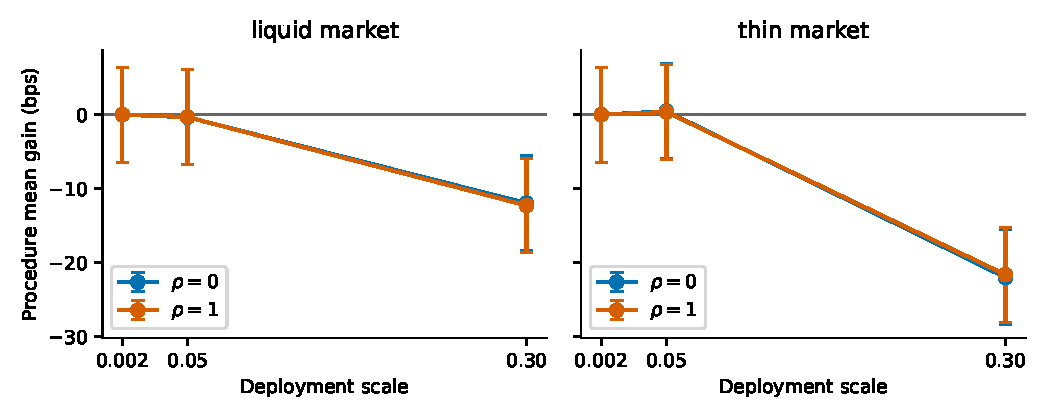
\includegraphics[width=.98\linewidth]{market_scale.pdf}
\caption{Procedure mean gain across the three tested order sizes under the original 100 bps utility. Error bars are approximate simultaneous 95\% bands for the full 24-estimate family, resampling all 50 roots jointly across both regimes. Lines connect observations and do not imply an interpolated capacity frontier.}\label{fig:scale}
\end{figure}
\begin{table}[t]\centering\small
\begin{tabular}{llrr}\toprule
Regime & $\rho$ & Mean & Simultaneous band \\
\midrule
Liquid & $0$ & $-11.9800$ & $[-18.3944,\,-5.5656]$ \\
Liquid & $1$ & $-12.2848$ & $[-18.6992,\,-5.8704]$ \\
Thin & $0$ & $-22.0073$ & $[-28.4217,\,-15.5929]$ \\
Thin & $1$ & $-21.6446$ & $[-28.0590,\,-15.2302]$ \\
\bottomrule\end{tabular}
\caption{Largest-scale procedure gains ($s=0.30$), in bps. The original 24-estimate family uses the prespecified 100 bps completion utility and all 50 shared roots.}\label{tab:largest}
\end{table}

The four largest-scale means in Table~\ref{tab:largest} are below zero throughout their original simultaneous bands. All four largest-minus-smallest scale contrasts are also negative in that family. This supports a bounded statement about the frozen procedure at the tested large order size, rather than a claim that large updates or large trades generally fail.

The two lower scales and all response and interaction contrasts remain unresolved. In particular, a negative estimate in both response conditions cannot establish that inventory response caused the loss. It also does not establish equivalent outcomes across response conditions: the contrast intervals permit differences in either direction. The complete family, including these unresolved contrasts, appears in Appendix~\ref{app:all24}.

At the smallest scale the paired gains are exactly zero in the saved paths: for this policy class, an initial aggressive slice can complete the small parent. The experiment consequently certifies no positive initial scale segment. Its upper bands fail to exclude positive values at the two lower scales, but that is weaker than evidence of a profitable operating region. There is no jointly supported positive-to-negative crossing and no estimated continuous capacity threshold.

Among the 49 adopted roots per regime, estimated root means at the largest scale reverse sign in 37 liquid-regime roots and 48 thin-regime roots at each response setting. These descriptive counts summarize how widespread the observed negative root means are. They do not enter the original 24-estimate mean family or supply a population risk bound. The root-level distribution and no-update zeros are shown in Appendix~\ref{app:root-diagnostics}.

\subsection{Proxy-to-deployment comparison at the selection scale}
As a separate post-outcome diagnostic, we compare the saved proxy gain of each selected candidate with its mean paired interactive-deployment gain at $s=0.05$, the scale used to score candidates. Both quantities use the recorded $U_{100}$ convention, and no-update roots contribute zero to both. For root $r$ and condition $z$, let $\Gamma_{r,z}=\Delta^{\rm proxy}_{r}-D_{r,z,0.05}$; Table~\ref{tab:proxy-deployment-gap} reports the four root-population means. All four estimated gaps are positive and their separate four-estimate simultaneous bands exclude zero. This contrast does not identify a causal proxy bias: it combines winner selection, finite proxy-sample noise, and differences between replay and interactive books. It reuses the original 50 roots and is outside the prespecified 24-estimate family.
\begin{table}[H]\centering\footnotesize
\begin{tabular}{llrrrr}\toprule
Regime & $\rho$ & Proxy & Deploy. & $\widehat\Gamma$ & Joint band \\
\midrule
Liquid & $0$ & 0.972 & -0.342 & 1.314 & $[0.649,\,1.979]$ \\
Liquid & $1$ & 0.972 & -0.322 & 1.294 & $[0.629,\,1.959]$ \\
Thin & $0$ & 1.422 & 0.470 & 0.952 & $[0.288,\,1.617]$ \\
Thin & $1$ & 1.422 & 0.365 & 1.057 & $[0.392,\,1.722]$ \\
\bottomrule\end{tabular}
\caption{Outcome-aware comparison at the $s=0.05$ selection scale, in bps under the recorded $U_{100}$ convention. Proxy, deployment, and gap means use all 50 roots; the final column gives the approximate simultaneous 95\% whole-root bootstrap band for the four paired proxy-minus-deployment gaps. No-update roots contribute zero. This auxiliary family is separate from the original 24-estimate family.}\label{tab:proxy-deployment-gap}
\end{table}


\subsection{Fixed-selection utility sensitivity}
The revaluation uses $p\in\{25,50,100,200\}$ and a separate 64-estimate family: 48 cell means and 16 largest-minus-smallest scale contrasts. It was specified after inspecting the primary outcomes. Twenty thousand shared-root bootstrap draws form its own simultaneous bands; it is neither a new independent experiment nor an expansion of the original confirmatory family.

\begin{figure}[t]\centering
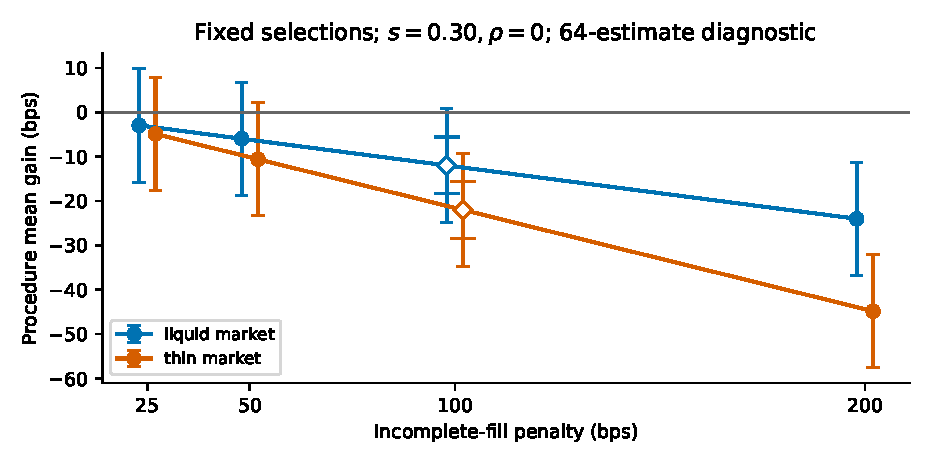
\includegraphics[width=.90\linewidth]{penalty_sensitivity.pdf}
\caption{Largest-scale fixed-selection revaluation for $\rho=0$. Filled markers use the 64-estimate diagnostic bands; open diamonds at 100 bps show the original 24-estimate bands. The point estimates coincide at 100 bps, while the joint uncertainty widths differ. All policies retain their original 100 bps selection.}\label{fig:penalty}
\end{figure}
\begin{table}[t]\centering\footnotesize
\begin{tabular}{llrrrr}\toprule
Regime & $\rho$ & $p=25$ & $p=50$ & $p=100$ & $p=200$ \\
\midrule
Liquid & $0$ & \shortstack{$-2.95$\\$[-15.74,\,9.83]$} & \shortstack{$-5.96$\\$[-18.74,\,6.82]$} & \shortstack{$-11.98$\\$[-24.76,\,0.80]$} & \shortstack{$-24.01$\\$[-36.80,\,-11.23]$} \\
Liquid & $1$ & \shortstack{$-2.75$\\$[-15.53,\,10.03]$} & \shortstack{$-5.93$\\$[-18.71,\,6.85]$} & \shortstack{$-12.28$\\$[-25.07,\,0.50]$} & \shortstack{$-25.00$\\$[-37.78,\,-12.22]$} \\
Thin & $0$ & \shortstack{$-4.88$\\$[-17.66,\,7.90]$} & \shortstack{$-10.59$\\$[-23.37,\,2.19]$} & \shortstack{$-22.01$\\$[-34.79,\,-9.23]$} & \shortstack{$-44.84$\\$[-57.63,\,-32.06]$} \\
Thin & $1$ & \shortstack{$-4.51$\\$[-17.30,\,8.27]$} & \shortstack{$-10.22$\\$[-23.01,\,2.56]$} & \shortstack{$-21.64$\\$[-34.43,\,-8.86]$} & \shortstack{$-44.48$\\$[-57.27,\,-31.70]$} \\
\bottomrule\end{tabular}
\caption{Largest-scale fixed-selection revaluation (bps), with approximate simultaneous 95\% bands for the separate, outcome-aware 64-estimate family. Each entry is a mean and its band; no selection is rerun.}\label{tab:penalty}
\end{table}

At 100 bps, the liquid-regime point estimates are unchanged but the 64-estimate bands include zero. The thin-regime means remain negative in that analysis. At 25 and 50 bps, all four largest-scale intervals include zero; at 200 bps, all four are below zero. Thus the original result should always name its utility and inferential family. One may not choose whichever family produces the desired significance interpretation after observing its result.

\subsection{Break-even completion preference: a separate diagnostic}
For fixed choices, write the population mean as $\mu_{\mathcal P}(z;p)=a_z+p b_z$, where $a_z$ is mean incumbent-minus-selected shortfall and $b_z$ is mean incumbent-minus-selected unfinished fraction. If $b_z\ne0$, its mathematical zero is $p_z^*=-a_z/b_z=-100a_z/d_z$, with $d_z=100b_z$ in percentage points. The estimate is the ratio of the two sample means, not the mean of root-specific ratios. It concerns revaluation of the same outcomes, not reselecting candidates at each penalty or locating a capacity threshold.

\begin{table}[t]\centering\small
\begin{tabular}{@{}lrrrrl@{}}\toprule
Regime & $\rho$ & $\bar a$ (bps) & $100\bar b$ (pp) & $\widehat p^*$ (bps) & Joint set, $p\geq0$ (bps)\\\midrule
Liquid & 0 & 0.0546 & -12.0346 & 0.454 & $[0.00,6.88]$\\
Liquid & 1 & 0.4295 & -12.7143 & 3.378 & $[0.26,18.24]$\\
Thin & 0 & 0.8292 & -22.8365 & 3.631 & $[2.38,5.36]$\\
Thin & 1 & 1.1958 & -22.8404 & 5.236 & $[3.60,7.50]$\\
\bottomrule\end{tabular}
\caption{Largest-scale completion-utility diagnostic with original choices fixed. The threshold is a ratio of mean components, $\widehat p^*=-\bar a/\bar b$, computed before rounding. The sets project an approximate simultaneous 95\% bootstrap rectangle for all eight component means, using 20,000 shared-root draws. This separate, outcome-aware family does not modify the original 24 or diagnostic 64 estimates.}\label{tab:break-even}
\end{table}

Table~\ref{tab:break-even} uses the unrounded root components. All four point estimates have positive shortfall gains and worse completion; their estimated zero crossings range from 0.454 to 5.236 bps. The small liquid-regime, response-off intercept is uncertain, so a positive crossing is not established in that cell. Shortfall improvement alone consequently does not determine the value of a procedure that changes completion.

Ratio uncertainty requires care. We resample all 50 roots jointly and construct a fixed-standard-error maximum-deviation rectangle for the eight component means, then project it onto $p\geq0$ where $a+pb=0$. The four resulting sets are bounded here, but the construction can return an unbounded or empty set. Each liquid cell has three denominator-sign changes among 20,000 draws; those draws remain in the component bootstrap and no percentile ratio interval is reported for those cells. Appendix~\ref{app:break-even} gives the construction and its limits. This outcome-aware eight-component family is separate from both earlier analyses; its intervals cannot replace their unresolved findings or be treated as new confirmation.

\subsection{Root sensitivity without new confirmation}
Post-outcome diagnostics remove each of the 50 roots in turn and reconstruct the original 24-estimate bands with 49 roots. Four additional constructions use two alternative random seeds, a standardized whole-root maximum, and a standardized Gaussian root-multiplier maximum. Their details and full outputs are supplied in Appendix~\ref{app:root-diagnostics}.

All four largest-scale upper bounds stay negative across these checks; the closest alternative upper bound to zero is $-3.13$ bps. This reduces concern that a single observed root or the tested resampling choices alone account for the original finding. It does not address misspecified liquidity, utility preferences, or other candidate classes. Because the diagnostics were chosen after the outcome and share the same data, no joint coverage is asserted across all methods or deletions, and no additional independent confirmation is claimed.

\section{Practical implications: a deployment assessment report}
The assessment specification can be used as a compact report schema for another frozen update procedure. It is a reporting and audit structure, not an automatic deployment gate. A report should bind the fields in Table~\ref{tab:report-schema} before interpreting outcome data and should assign a separate identity to any outcome-aware diagnostic.

\begin{table}[t]\centering\small
\begin{tabular}{@{}p{.19\linewidth}p{.34\linewidth}p{.36\linewidth}@{}}\toprule
Field & Required declaration & Market instantiation\\\midrule
Procedure & Candidate generation, selection rule, incumbent & Frozen generator; 16 candidates; replay-proxy winner\\
Adoption & Replacement gate and no-update behavior & Adopt only above $10^{-9}$ bps; retain incumbent otherwise\\
Population & Independent unit and target population & 50 shared generation roots; 100 root--regime decisions\\
Deployment & Environment, scale, and response conditions & Synthetic matching engine; two regimes, three scales, two responses\\
Utility & Outcome terms and preference parameters & $-S-pf$; primary $p=100$ bps\\
Costs & Research and operational costs included? & Not measured: compute, API/token use, latency, safety, or long-horizon failure costs\\
Evidence & Inferential family and sensitivity identity & 24-estimate bands; separate 64-estimate, proxy-gap, and break-even diagnostics\\
Interpretation & Positive, negative, unresolved, and exclusions & Sign classification for the declared procedure mean\\\bottomrule
\end{tabular}
\caption{Procedure-level deployment assessment report schema. The final column records this study's choices; another application must supply its own procedure, population, utility, and evidence family.}\label{tab:report-schema}
\end{table}

The evidence labels in Table~\ref{tab:evidence} are useful only relative to the declared utility and inferential family. Positive evidence for a procedure mean does not establish acceptable tail risk or safe deployment, and an unresolved cell is an evidence gap rather than evidence of zero value. The bounded planner-code case is retained in the Supplementary Material as an auxiliary example with three generation roots and a fixed task panel; it is not pooled with the market cohort or used to claim agent generalization.

For future applications, a net utility could subtract research and operations costs, for example $V_{\rm net}=\mu_{\mathcal P}-\lambda_c C_{\rm compute}-\lambda_t C_{\rm latency}-\lambda_r C_{\rm risk}$. The present study does not observe these terms, so it reports deployment utility conditional on the declared execution preference rather than a net economic value.

\section{Discussion and reproducibility}
\subsection{Implications for machine-learning deployment evaluation}
The results illustrate why deployment utility is a property of a specified update-selection procedure rather than an intrinsic property of a proxy score or selected policy. The same frozen procedure can receive different assessments when operating conditions or completion preferences change. A deployment claim is also inseparable from its inferential target: repeated evaluations within a root do not replace independent update decisions, and a wider inferential family can leave a previously resolved conclusion uncertain.

This perspective is relevant to policy-learning and iterative optimization systems beyond the execution setting studied here. Extending it to coding agents, autonomous research systems, or other operational environments requires independently frozen procedures, domain-appropriate utilities, explicit cost and failure terms, and new evaluation populations. The current market evidence does not establish that the same effects occur in general-purpose agents.

\paragraph{What the release reproduces.}
The anonymous package contains normalized saved observations, pinned numeric references, source/protocol identifiers, and manuscript sources. Its single wrapper recomputes the 24- and 64-estimate analyses, break-even diagnostic, root audits, and supplementary planner summaries before generating tables and vector figures and compiling the paper. Numeric differences are checked within $10^{-9}$ in native units. The package is tested by extraction into a separate directory and execution in an isolated environment; rebuilding PDF bytes is not the criterion because rendering metadata can differ.

This is saved-outcome reanalysis. It does not regenerate model proposals, re-fit the classification tasks from original datasets, or reconstruct all exchange episodes. Those earlier raw-record and grade audits have separate receipts. Successful reanalysis establishes arithmetic and packaging reproducibility, while an external rerun of the original scientific processes remains a stronger test. Failure evidence and incomplete studies in the wider project are preserved but are not evidence for the current claims.

\section{Limitations and operational scope}
\paragraph{Statistical limits.}
The independent-market root population is finite in this sample and synthetic in its definition. The bootstrap supplies approximate conditional joint uncertainty, not exact coverage or simulator-model uncertainty. The adopted-root sign counts additionally reflect finite deployment replication. Utility revaluation and root diagnostics are outcome-aware. No selection-policy comparison at alternative penalties, market search-pressure effect, monotone scaling law, or equivalence of response conditions is established.

\paragraph{External validity.}
The matching engine's priority rules do not make the surrounding market realistic. Provider refresh, depth, and inventory response follow a designed model; persistent execution queues, institutional constraints, and real own-order impact are unvalidated. The experiment does not justify professional trading or calibration to a particular crypto venue. The planner case covers bounded edits and a fixed task panel, with no independent model-backbone replication or completed primary autonomous-agent study.

The assessment does not measure API costs, token consumption, computational latency, agent safety, or long-horizon reliability. Completion utility is an explicit preference over execution outcomes, not a surrogate measurement of these other dimensions. Referencing broader deployment-evaluation work does not make them part of the present evidence.

\paragraph{Practical use.}
A deployment report should name the procedure being assessed, retain no-update decisions, declare utility before interpreting value, and present uncertainty over the actual intended claim. Positive evidence on a tested grid still leaves operational failure severity and deployment conditions to be assessed. Conversely, unresolved cells are evidence gaps, not proof of zero benefit. Any future extension to a real workflow requires a separately frozen evaluation and appropriate cost and failure accounting; this paper provides no ready-made authorization for deployment.

\section{Conclusion}
This study evaluates the deployment utility of a frozen policy-update procedure rather than the isolated proxy performance of a selected candidate. Its central finding is conditional: under one synthetic execution environment, prespecified completion preference, and original joint inferential family, the procedure has negative mean utility at the largest tested order size. Lower-scale cells and response contrasts remain unresolved. Fixed-selection revaluation demonstrates that utility preferences and inferential scope must accompany any deployment statement, while the break-even analysis provides an explicitly post-outcome characterization of the same saved outcomes. A separate selection-scale diagnostic finds positive proxy-minus-deployment gaps across all four regime--response cells, but its outcome-aware construction cannot identify a causal proxy-bias effect.

The methodological implication is to distinguish the value of an individual update from the expected utility of the complete procedure that generates and adopts updates. A defensible assessment retains incumbent decisions, declares operating conditions and utility, identifies independent evaluation units, and aligns statistical evidence with the intended claim. The formal properties supplied here are reusable characterizations, not a universal deployment theorem or a new fidelity algorithm.

The evidence is conditional on one frozen synthetic market and one update procedure. It does not establish general agent reliability, professional-market execution validity, a universal scaling law, or net value after compute and operational costs. Independent simulators, alternative update procedures, and autonomous-agent populations remain necessary for broader validation.

\paragraph{Author contributions and AI assistance.}
The authors conducted the research and prepared the manuscript, with limited AI assistance in drafting and code preparation.

\bibliographystyle{style/tmlr}
\bibliography{references}
\appendix

\section{Protocol details and provenance}\label{app:protocol}
The engine revision is \texttt{f94150294a85d7b415ca4518590b5a661d6f9958}. It uses integer prices, quantities, and microsecond event times. Fundamental innovations are $-1,0,+1$ ticks with probabilities $0.25,0.50,0.25$. Provider quote centers add
\[
\operatorname{clip}\!\left(-\operatorname{round}\left\{2\rho\,[I_j(t)-I_j(120)]/100\right\},-8,8\right)
\]
ticks to the current fundamental price; rounding is ties-to-even. All actor cash and inventory begin at zero, with shorting and negative cash explicitly permitted. This convention is part of the simulation, not an account-risk model.

The event phases order fundamental changes, provider refreshes, background takers, activation, proxy snapshots, and execution children. Provider refresh cancels residual orders and inserts the fixed ladder. Limited-price execution children cancel any unfilled residual within the atomic operation. Separate cash/inventory ledgers attribute both sides of each fill. The retained events support checking cancellations against actual remaining quantity and reconstructing book state without invoking the upstream matcher.

Calibration and engineering roots are separate from the 50 prospective roots, locally labeled 8101--8150 within cohort \texttt{cohort-20260930-v1}. Regime-specific expected volumes come from 40 calibration paths per regime. The protocol fixes eight proxy paths and four deployment paths per root/regime. Paired deployment paths share exogenous innovations and arrival states, while policies and resulting endogenous event paths may differ. Exact-zero and small-scale checks test the implementation's boundary behavior and are not substitutes for new independent roots.

The labels 8101--8130 also appear as seeds in the earlier PIVOT E2C cohort and are not globally unique root identifiers. PIVOT E2C uses NumPy \texttt{default\_rng} for candidate and environment draws. Here candidate perturbations use Python \texttt{random.Random}; deployment streams use SHA-256-derived seeds namespaced by cohort, root, split, replicate, actor, and channel before using \texttt{random.Random}. The submitted PIVOT data and figure files have no byte-identical matches to the current outcome files and figures. The shared integer labels therefore do not identify shared saved outcomes; the distinct cohort protocols, rather than label novelty, define the current sample.

The 100 bps completion preference, policy equations, and candidate perturbations were carried forward from development to maintain a fixed comparison. The new exchange lineage, prospective roots, and source freeze distinguish the principal cohort from those development trials. They do not establish independence from every design decision informed by development. The prior PIVOT supplement's virtual finance fixtures use a different execution construction and are not reported as current results.

The supplemental provenance inventory identifies the original protocol and the saved inputs used by the portable release. The actual ICLR main manuscript and its submitted ZIP are the related-work comparison baseline, alongside the public preprint. Their identities are retained internally; the anonymous main manuscript is included only as comparison material. Reuse of a statistical tool with attribution is distinguished from reporting an existing empirical result as a new contribution.

\section{Complete original inferential family}\label{app:all24}
Table~\ref{tab:all24} preserves the full prospective family. The four scale contrasts subtract the smallest-scale cell from the largest-scale cell within each regime and response setting. Response contrasts subtract $\rho=0$ from $\rho=1$ at a fixed scale. An interaction subtracts the $\rho=0$ scale contrast from the $\rho=1$ scale contrast. All share the same root resampling and maximum-deviation radius.
\begin{table}[t]\centering\small
\begin{tabular}{llrr}\toprule
Regime & Estimand & Mean & Simultaneous band \\
\midrule
Liquid & Cell: $\rho=0, s=0.002$ & $0.0000$ & $[-6.4144,\,6.4144]$ \\
Liquid & Cell: $\rho=0, s=0.05$ & $-0.3420$ & $[-6.7564,\,6.0724]$ \\
Liquid & Cell: $\rho=0, s=0.3$ & $-11.9800$ & $[-18.3944,\,-5.5656]$ \\
Liquid & Cell: $\rho=1, s=0.002$ & $0.0000$ & $[-6.4144,\,6.4144]$ \\
Liquid & Cell: $\rho=1, s=0.05$ & $-0.3219$ & $[-6.7363,\,6.0925]$ \\
Liquid & Cell: $\rho=1, s=0.3$ & $-12.2848$ & $[-18.6992,\,-5.8704]$ \\
Thin & Cell: $\rho=0, s=0.002$ & $0.0000$ & $[-6.4144,\,6.4144]$ \\
Thin & Cell: $\rho=0, s=0.05$ & $0.4695$ & $[-5.9449,\,6.8839]$ \\
Thin & Cell: $\rho=0, s=0.3$ & $-22.0073$ & $[-28.4217,\,-15.5929]$ \\
Thin & Cell: $\rho=1, s=0.002$ & $0.0000$ & $[-6.4144,\,6.4144]$ \\
Thin & Cell: $\rho=1, s=0.05$ & $0.3650$ & $[-6.0494,\,6.7794]$ \\
Thin & Cell: $\rho=1, s=0.3$ & $-21.6446$ & $[-28.0590,\,-15.2302]$ \\
Liquid & Scale: $\rho=0$ & $-11.9800$ & $[-18.3944,\,-5.5656]$ \\
Liquid & Scale: $\rho=1$ & $-12.2848$ & $[-18.6992,\,-5.8704]$ \\
Thin & Scale: $\rho=0$ & $-22.0073$ & $[-28.4217,\,-15.5929]$ \\
Thin & Scale: $\rho=1$ & $-21.6446$ & $[-28.0590,\,-15.2302]$ \\
Liquid & Response: $s=0.002$ & $0.0000$ & $[-6.4144,\,6.4144]$ \\
Liquid & Response: $s=0.05$ & $0.0201$ & $[-6.3943,\,6.4345]$ \\
Liquid & Response: $s=0.3$ & $-0.3048$ & $[-6.7192,\,6.1096]$ \\
Thin & Response: $s=0.002$ & $0.0000$ & $[-6.4144,\,6.4144]$ \\
Thin & Response: $s=0.05$ & $-0.1046$ & $[-6.5190,\,6.3098]$ \\
Thin & Response: $s=0.3$ & $0.3627$ & $[-6.0517,\,6.7771]$ \\
Liquid & Scale-by-response & $-0.3048$ & $[-6.7192,\,6.1096]$ \\
Thin & Scale-by-response & $0.3627$ & $[-6.0517,\,6.7771]$ \\
\bottomrule\end{tabular}
\caption{All 24 prospective estimates in bps, using one shared-root maximum-deviation band. Scale denotes $0.30-0.002$; response denotes $1-0$. Unresolved contrasts are retained.}\label{tab:all24}
\end{table}


\section{Post-outcome root diagnostics}\label{app:root-diagnostics}
\subsection{Construction and deletion results}
\label{app:root-robustness}
These checks reuse the frozen selections and 100 bps utility after the original outcomes were inspected. They neither add independent roots nor extend the original confirmatory family. Each method resamples the complete root vector across both regimes and all 24 estimands.

\begin{table}[h]\centering\small
\begin{tabular}{llrrr}\toprule
Regime & $\rho$ & LOO mean range & Max. LOO upper & Max. alternative upper\\\midrule
Liquid & 0 & [-13.26, -11.49] & -4.98 & -3.13\\
Liquid & 1 & [-13.50, -11.78] & -5.30 & -3.62\\
Thin & 0 & [-23.01, -21.83] & -15.28 & -15.61\\
Thin & 1 & [-22.63, -21.47] & -14.92 & -15.25\\
\bottomrule\end{tabular}
\caption{Largest scale $s=0.30$: all values are bps. Leave-one-root-out (LOO) checks refit a 24-estimate unstandardized maximum-deviation band using 49 shared roots and 20,000 draws for each of 50 deletions. Alternative bounds use two independently seeded paired-root runs, a fixed-sample-SE standardized paired-root maximum, and a standardized Gaussian root-multiplier maximum, each with 20,000 draws. No joint coverage is claimed across methods or deletions.}\label{tab:root-robustness}\end{table}

Standardization divides bootstrap deviations by the original sample standard error, not a reestimated standard error in each draw. Gaussian multipliers approximate the centered root-mean distribution using its empirical covariance. Constant observed columns are flagged; a zero empirical standard error does not establish zero population uncertainty. Numerical bands remain approximate and conditional on the frozen synthetic world.

\begin{figure}[h]\centering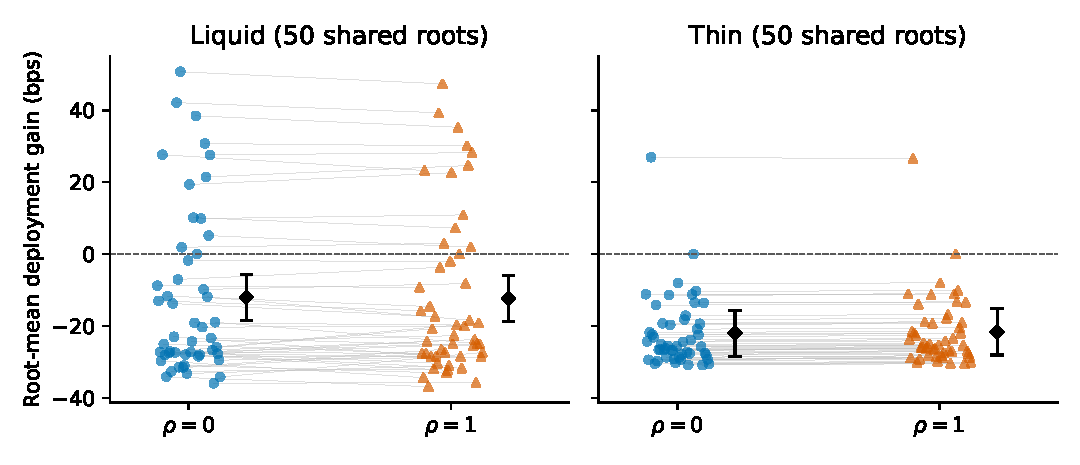
\includegraphics[width=.95\linewidth]{market_root_distribution.pdf}
\caption{Fifty root-level procedure gains at the largest scale under the original 100 bps utility. Each point averages four paired deployments; lines connect the same root across response settings. Incumbent-retaining roots contribute zero. Diamonds and bars show the original full-cohort means and 24-estimate simultaneous bands, not uncertainty for individual roots.}\label{fig:root-distribution}\end{figure}

The standardized maximum uses the original sample standard error for each estimand, not a standard error recomputed within every bootstrap draw. The Gaussian multiplier draws centered root vectors with conditional mean-distribution covariance matched to the sample covariance divided by the root count. These alternatives probe particular construction choices. They are not independent replications, and reporting the greatest upper bound among the checks does not create a new simultaneous confidence procedure.

\section{Break-even diagnostic construction}\label{app:break-even}
The November 4 diagnostic specification records that the v5 outcomes and component means had already been inspected. At $s=0.30$, each root contributes $(a_{r,j},b_{r,j})$ for each of the four regime--response cells $j$, averaging its four paired repetitions and retaining no-update zeros. Let $X_r\in\mathbb R^8$ collect these components, and let $\widehat\sigma_k$ be each sample mean's standard error. Twenty thousand common root resamples, using PCG64 seed 20261104, give the 95th percentile of
\[
\max_{k\leq8}\frac{|\overline X_k^{(b)}-\overline X_k|}{\widehat\sigma_k}.
\]
The critical value is 2.512769. The denominators are the original sample standard errors, not bootstrap-specific estimates. All eight empirical variances are positive; the implementation rejects constant components rather than treating zero empirical variation as known population certainty.

For a cell's rectangle $[a_L,a_U]\times[b_L,b_U]$, the projected set is
\[
\mathcal C_j=\{p\geq0:a_L+p b_L\leq0\leq a_U+p b_U\}.
\]
This inversion uses the affine utility and preserves unbounded or empty sets when the data permit them. Conditional on coverage of the eight-component rectangle, every existing nonnegative zero of those covered mean utilities belongs to its projected set. Coverage is approximate and conditional on the synthetic population; a nonempty projected set does not prove that a nonnegative zero exists. The nominal level treats this diagnostic specification as given and does not adjust for choosing it after inspecting outcomes. The rectangle discards some within-cell covariance geometry during projection, so the sets can be conservative. No joint guarantee is asserted across this analysis and the earlier 24- or 64-estimate families.

For both liquid cells, three resampled denominators change sign; none is zero. For both thin cells, neither event occurs. The report retains these counts, all draws in the component construction, and the untrimmed pointwise percentile ratios for the two stable thin cells (3.113--4.151 and 4.702--5.768 bps). Those narrower pointwise summaries are not the joint sets in Table~\ref{tab:break-even}. The liquid, response-off intercept rectangle includes zero and negative values; its displayed $[0,6.88]$ set therefore does not establish a positive-to-negative population crossing. These choices follow the separate outcome-aware diagnostic specification and do not change the frozen original analysis.

\section{Adoption and utility interpretation}
Equations~\ref{eq:root-gain}--\ref{eq:adoption-identity} separate a procedure's expected gain from the outcomes of its adopted subset. Conditioning on observed deployment outcomes to decide adoption would change the estimand and invalidate the stated gate. Here selection is closed before those outcomes. Changing the utility coefficient while holding selection fixed is also distinct from reevaluating a procedure that would optimize the new coefficient.

In particular, a positive conditional gain given adoption can coexist with a small procedure mean when adoption is rare; a given reversal rate can coexist with either positive or negative value depending on the loss magnitudes. Neither fact is offered as a new theorem. These accounting distinctions specify what a saved-outcome analysis can answer. Missing, failed, or altered root records must not be silently converted to no-update zeros; the portable checks reject incomplete identities and nonfinite outcomes.
\end{document}
